\section{Experiments Results for Independent tasks}
\label{sec:experiemnts}

In the previous section, we proved a new upper bound of the Makespan
of WS with an explicit latency. The objective of this section is to
study WS experimentally in order to confirm the theoretical results
and to refine the constant $\gamma$. To this end, we developed an
\textit{ad-hoc} simulator that follows strictly the WS model. We focus on
the case of independent tasks. We start by describing this
simulator and the considered test configurations.  Using the
experimental results, we show that the previous theoretical bound is close to
the experimental results.  We conclude with a discussion on where
would the analysis be made more precise. 
%OFinally, we discuss different difficulties of our analyze and the constant factor $4\gamma$ of the $\log_2(\frac{\mathcal{W}}{\lambda})$.


\subsection{Simulator}

Simulation analysis is a very popular and powerful method 
for understanding complex problems when mathematical analysis is unreachable.

For this purpose, there exist many simulators on parallel and distributed computing.
Most of them are developed for specific research projects by researchers and are not well-documented,
and/or no longer maintained. However, there exist several general purpose and high quality simulators
like SimGrid~\cite{SIMGRID} that includes many features: It allows to consider complex
situations like congestion, cache effects for particular architectures, etc.
However, such simulators are usually very computationally expensive,
and it requires a high entry cost to develop in.

Our purpose here is less ambitious since we target simple processing
units. We are interested in observing a simple aspect of the execution process of WS
algorithms on platforms with different topologies.
For these reasons, we developed a lightweight simulator,
%which was designed to be sufficiently flexible in order to simulate different Work Stealing models.
Its flexibility allows us to experiment several variants of WS algorithms,
with different topologies, and different types of application.
The simulator generates also extensive logs for a detailed analysis for each tested scenario.

WS-simulator can run different models of execution under the WS paradigm of an application on a platform. An application
consists of a list of tasks with or without dependencies, and the
platform consists of multiple processors linked by a specific
network/topology.  The simulator allows to execute a scenario with a specific
task on a specific platform. 

The overall architecture of WS-Simulator is composed of six main units (called engines),
that are depicted in Figure~\ref{fig:archsimu}. The event engine is the core of the simulator,
it manages the processors' events during the time to run the simulation of a scenario.
The events are executed through the processor engine, which provides different
functionalities to perform the tested WS algorithm.
The processor engine uses the task engine to manage the execution of the tasks
and it uses the topology engine to manage the interactions between the processors.
During the execution of a simulation, the log engine keeps track of different
information and generates different logs.
More details are available at the website \url{https://wssimulator.github.io}
which describes in detail our simulator and how to use it.

\begin{figure}[h]
  \centering
    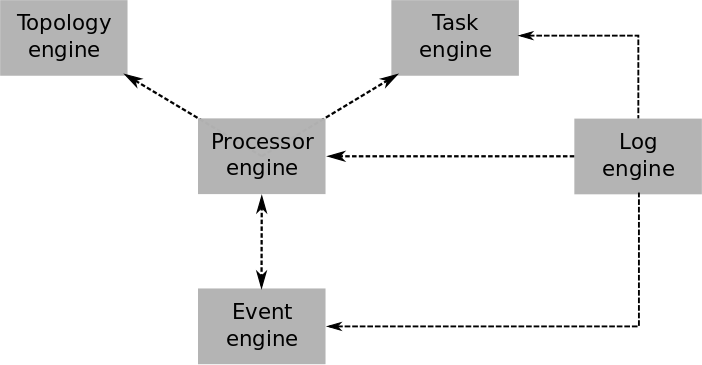
\includegraphics[width=0.7\linewidth]{figures/simulatorArchitecture.png} 
  \caption{The overall architecture of WS-simulator}
    \label{fig:archsimu}
\end{figure}


\subsection{Configurations}

For our tests, we configure our WS-simulator in order to follow the model
of independent tasks described in Section~\ref{sec:wsmechanisms} to
schedule $\mathcal{W}$ unitary independent tasks on a distributed
platform composed of $p$ identical processors. The communication
latency between the processors is equal to $\lambda$.  
To ensure reproducibility, this configuration of the simulator is detailed
in WS-Simulator website\footnote{\url{https://wssimulator.github.io/pages/wssimulator-one-cluster.html}}.

\subsection{Validation of the bound and definition of the ``overhead
  ratio''}

% under different parameters $\mathcal{W}$, $p$ and $\lambda$. 


As seen before, the bound of the expected Makespan is the sum of two
terms: The first term is the ratio $\mathcal{W}/{p}$ which does not
depend on the configuration nor on the algorithm; The second term
represents the overhead related to work requests.  Our analysis bounds
the second term to derive our bound on the Makespan.  To analyze the
validity of our bound, we define what we call the \emph{overhead
  ratio} as the ratio between the second term of our theoretical bound
($4\gamma\lambda\log_2(\mathcal{W}/\lambda)$) and the simulated
execution time minus the ratio $\mathcal{W}/p$: for a given
simulation, we define
\begin{align}
  \label{eq:overhead}
  \text{Overhead\_ratio}=\frac{4\gamma\lambda\log_2(\mathcal{W}/\lambda)}
  {\text{Simulated\_execution\_time}  - \frac{\calW}{p}}.
\end{align}

To study this overhead ratio, 
%As said earlier, each simulation is fully described by three
%parameters: $(\calW, p, \lambda)$. For our tests, 
we vary the number of unit tasks $\mathcal{W}$ between $10^5$ and $10^8$, the number of
processors $p$ between 32 and 256 and the latency $\lambda$ between 2
and 500 which is a realistic range of actual systems.
Each experimental setting has been reproduced 1000 times in
order to compute median or interquartile ranges. 


\begin{figure}[ht]
  \centering
  \begin{tabular}{@{}c@{}c@{}c@{}}
    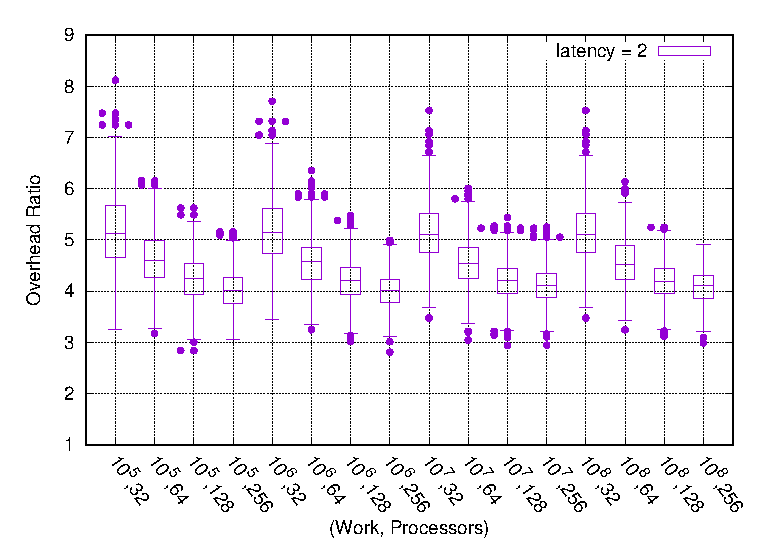
\includegraphics[width=0.33\linewidth]{figures/overheadratioWPinv2.eps}
    
    % \caption{Overhead ratio as a function of $(\mathcal{W},p)$  ($\lambda = 262$)}
    % \label{fig:accuracy}
    % \end{figure}
    % \begin{figure}[tp!]
    %   \centering
    &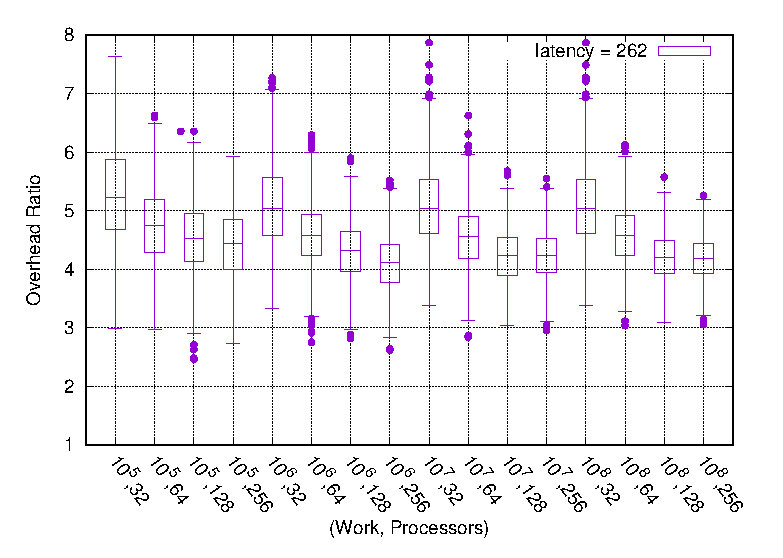
\includegraphics[width=0.33\linewidth]{figures/overheadratioWPinv262.eps}
    &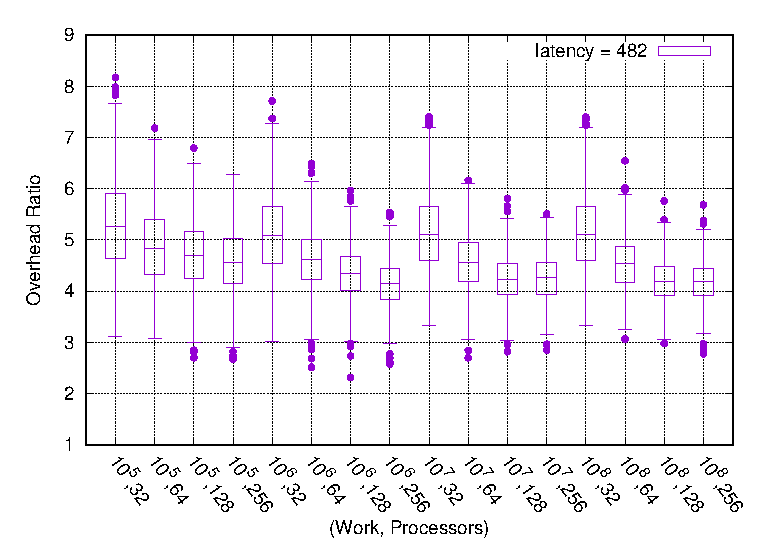
\includegraphics[width=0.33\linewidth]{figures/overheadratioWPinv482.eps}\\
    (a) Latency $\lambda=2$
    &(c) Latency $\lambda=262$&(d) Latency $\lambda=282$
    
  % \caption{Overhead ratio as a function of $(\mathcal{W},p)$   ($\lambda = 262$)}
%  \label{fig:accuracy}
%\end{figure}
%\begin{figure}[tp!]
%  \centering
  
  
  \end{tabular}
    
  \caption{Overhead ratio (defined in Equation~\eqref{eq:overhead}) as
    a function of $(\mathcal{W},p)$ for different values of
    latency~$\lambda$.}
  \label{fig:accuracy}
\end{figure}


%\begin{figure*}[!t]
%\centerline{\subfigure[Case I]{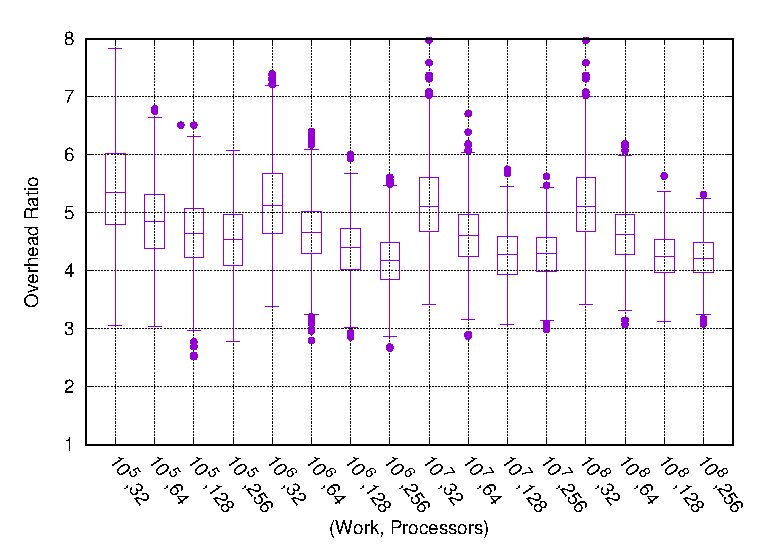
\includegraphics[width
%=2.5in]{figures/overheadratioWPinv.eps}
%%\label{fig_first_case}}
%%\hfil
%%\subfigure[Case II]{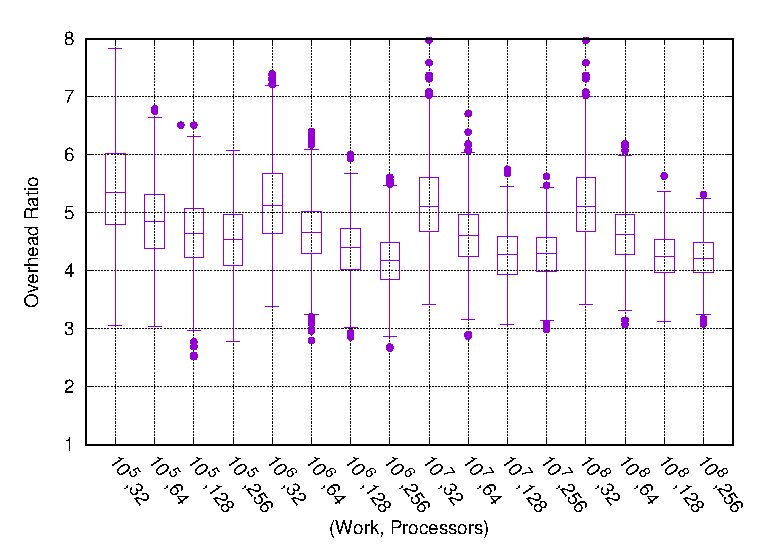
\includegraphics[width=2.5in]{figures/overheadratioWPinv.eps}
%%\label{fig_second_case}}}
% \caption{Simulation results}
%\label{fig_sim}
%\end{figure*}



Figure~\ref{fig:accuracy} plots the overhead ratio according to each
couple $(\mathcal{W}, p)$, for different latency values $\lambda= \{2,\ 262,\ 482\}$
units of time.
%Similar observations have been observed with all values of latency used.
The~x-axis is $(\mathcal{W}, p)$ for all values of $\mathcal{W}$ and $p$ intervals
and the y-axis shows the overhead ratio.
We use here a BoxPlot graphical method to present the
results. BoxPlots provides a good overview and a numerical summary of a
data set.  The ''interquartile range'' in the middle part of the plot
represents the middle quartiles where 50\% of the results are
presented.  The line inside the box presents the median. The whiskers
on either side of the IQR represent the lowest and highest quartiles
of the data.  

We observe that our upper bound is about 4 to 5.5 times greater than
to the one computed by simulation (depending on the range of
parameters). The ratio between the two bounds decreases with the
number of processors but seems fairly independent of $\calW$.


\begin{figure}[htb]
  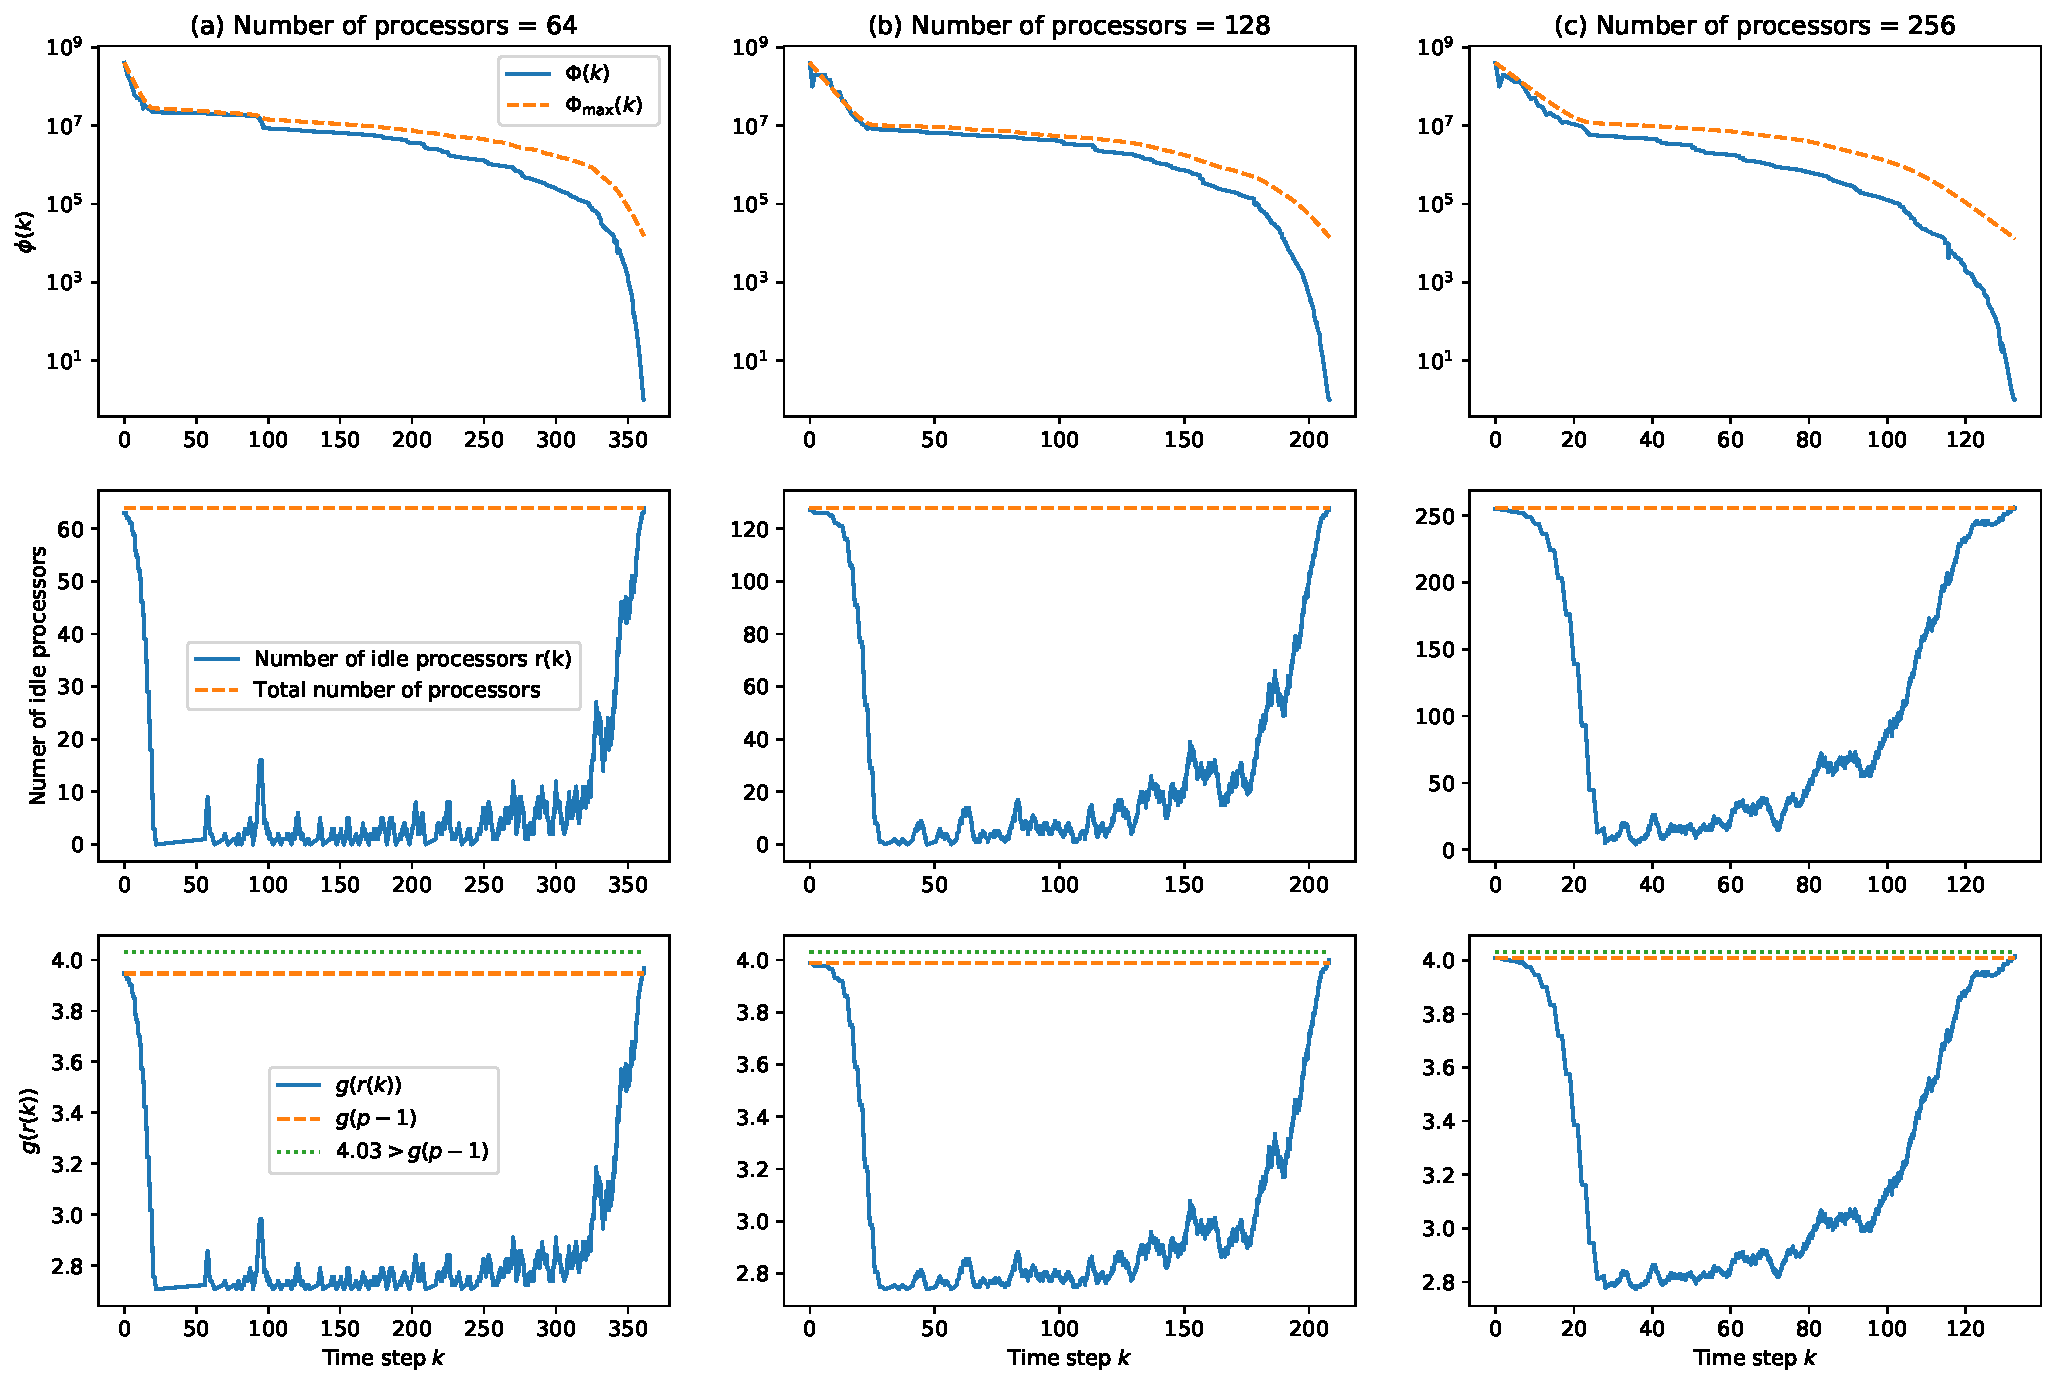
\includegraphics[width=\linewidth]{figures/analysis.pdf}
  \caption{Evolution of the state of the systems for different
    number of processors ($\lambda=500,\ W=10^7$). Each column
    corresponds to a number of processors ($64$, $128$ or
    $256$).  The first line corresponds to $\phi_{\max}$
    (defined in Equation~\eqref{eq:phi_max}).  The second line
    displays the number of idle processors $r(k)$. The third
    line displays $g(r(k))$ (defined in
    Equation~\eqref{eq:g}). In all figures, the $x$-axis
    corresponds to the number of time steps $k$.}
  \label{fig:exp_analysis}
\end{figure}

\subsection{Discussion : where does the overhead ratio come from?}

The challenge of this paper is to analyze WS algorithm with an
explicit latency.  We presented a new analysis which derives a bound
on the expected Makespan for a given $\mathcal{W}$, $p$ and~$\lambda$.
It shows that the expected Makespan is bounded by $\calW/p$ plus an
additional term bounded by $4\gamma\lambda\log_2(\calW/\lambda)$ with
$4\gamma\approx16$.  As observed in Figure~\ref{fig:accuracy}, the
constant $4\gamma$ is about four to five times larger than the one
observed by simulation. A more precise fitting based on simulation
results leads to the expression
$\mathcal{W}/p + 4\lambda\log_2(\mathcal{W}/\lambda)$ (the value $4$
is an average over all our experiments). We explain below where does
the discrepancy between the theoretical bound of $16$ and the
experimental result of $4$ come from by looking at the different steps
of the proof.  Our analysis makes essentially three approximations:
-1) The function $h(r)$ is an upper bound on the potential diminution.
-2) We consider a worst case scenario for the number of steal requests
when we define $\gamma=\max_rg(r)=g(p-1)$; and (3) We bound $\gamma$
by $4.03$.  We review below the contribution of each approximation to
the overhead ratio.

To illustrate our explanations, we run three simulations by using our
simulator and report the results in Figure~\ref{fig:exp_analysis}.
These three executions have the same number of tasks $W=10^7$ and
latency $\lambda=500$ and we consider three values of processors:
$p\in\{64,\ 128,\ 256\}$. This figure illustrates the evolution with
time of the potential $\phi(k)$, the number of idle processors and the
value of $\gamma$ defined in section~\ref{gamma}. Each column
represents a value of $p$.  The lines represent the results for each
metric.


% Now, we briefly review the different approximation in order to explain
% the role of each approximation in the overhead ratio.

\subsubsection{Impact of the bound $h(r)$}
The first step of our analysis is to prove a bound on the decrease
potential: We show in Lemma~\ref{lem:indep} that
\begin{align}
  \label{eq:phi_exp}
  \esp{\Phi(k+1) \mid \calF_t} \le h(r(k)) \Phi(k). 
\end{align}

This bound is obtained by computing the diminution of the potential in
the various cases of the proof of Lemma~\ref{lem:indep}.  These various
cases make different approximations. First, our bound $h(r)$ is the
maximum between the ratio $2/3$ of Case~1 and the 
ratio $h(r)$ of Case~2a. Second, we assumed that we do not know when a
work requests arrive in the interval.  We therefore always took the
worst case (arrivals at the end of the intervals). Third, we neglect
the diminution of the potential due to working processors (Case~2a).

To see measure the impact of this approximation, we define a
theoretical function $\phi_{\max}(k)$ that would corresponds to the
potential of the system if the inequality of
Equation~\eqref{eq:phi_exp} was an equality:
\begin{equation}
  \label{eq:phi_max}
  \phi_{\max}(k) =
  \begin{cases*}
    \phi(0) & if $k = 0$, \\
    h(r(k))\phi_{\max}(k-1)        & otherwise.
  \end{cases*}
\end{equation}

In Figure~\ref{fig:exp_analysis}-(Line~1), we plot this theoretical
function and the real potential function as a function of time step
$k$. This figure indicates that the distance between the real
potential and the theoretical bound is relatively small at the
beginning of the execution, which makes sense since the diminution of
the potential is dominated by the diminution related to Case~2a. The
two function starts diverging slowly in the middle of the execution
and this divergence is accentuated at the end: when the execution is
close to finishing, the actual potential decreases much faster that
its bound. We believe that this divergence is mostly due to neglecting
the diminution of potential due to working processors: At the
beginning of the execution when all processors have many tasks to
execute, neglecting working processors is negligible; At the end of the
execution when the remaining work is small, the potential diminution
is greatly affected by the working processors.  Our analysis could be
tightened by taking a more complex potential function that will take
more carefully the impact of working processors.
% We do not believe, however, that there is an easy way to do so.

\subsubsection{Evolution of the number of work requests}

In our analysis, we study how the potential decreases a function of
the number of steal requests $r(k)$. To obtain a bound, we then use a
worst-case analysis and define $\gamma$ as the maximal of a function
$g(r)=r/(-p\log_2h(r))$: $\gamma=\max_r g(r)$. As shown in
Figure~\ref{fig:g}, $g(r)$ is between $2.8$ where $r$ is small to $4$
when $r$ is large.  On the second Line~2 of
Figure~\ref{fig:exp_analysis}, we depict how the number of idle
processors evolve over time. We observe that an execution has
essentially three phases: At the beginning, there is a high number of
idle processors since the work has to be divided among processors; In
the middle of the execution, the number of idle processors is small as
everybody is working.  In the final execution phase, it increases as
finding work becomes harder.


In Figure~\ref{fig:exp_analysis}-(Line~3), we plot $g(r(k))$ and
$\gamma$ as a function of the time step $k$.  The figure shows that
$g(r(k))$ is often about $2.8$ (because the period where the number of
idle processors is low is long). This suggests that our bound
$\gamma=\max_r g(r)$ is about $1.4$ times too high. Being able to
capture more precisely how the number of idle processors evolves might
lead to a bound that would be around $30\%$ times smaller.

\subsubsection{Bound $\gamma<4.03$ and impact of the number of
  processors}

In our analysis, we show that $\gamma=g(p-1)$ and we bound $\gamma$ by
$4.03$. In fact, the value of $4.03$ corresponds to what happens when
$p$ goes to infinity but smaller values of $p$ leads to smaller values
of $\gamma$. This explains why in Figure~\ref{fig:accuracy}, we
observe that the overhead ratio decreases with the number of processors,
from around $5$ for $32$ processors to around $4$ to $4.5$ for $256$
processors.


\medskip

In our simulation, we observe that the overhead ratio is between $4$
to $5$. Based on our experimental study of the evolution of the number
of work requests with time, we believe that the worst-case analysis
$\gamma=g(p-1)$ and the bound of $4.03$ contributes to a factor of
about $1.5$ of the overhead ratio. The remaining factor (of about $3$)
is mostly due to the bound $h$ that we obtained in
Lemma~\ref{lem:indep}. Refining this lemma, for example by being able
to estimate the decrease of potential due to the work execution or by
using a different potential definition, would lead to a tighter bound.




%%% Local Variables:
%%% mode: latex
%%% TeX-master: "main"
%%% End:
